%%% Results %%%
\chapter{Results} \label{ch:results}
\section{XY model on SAWs, 2D}
\subsection{Tests for validation simulations}
To test our Monte-Carlo (M) simulation, we compare results obtained using MC and Sampling + Exact Enumeration. For short chains ($N=5, N=8$), we generate all set of self-avoiding walks and sample spin configurations by uniform distribution $U(-\pi, \pi)$. As this is resource-consuming procedure, we sample spin configurations only $600$ times (so, 600 sequences of spins applied to each conformation) and repeat this $10$ times. Figure \ref{fig:ee} shows obtained results. This method is not reliable, but it helps to make approximate checks. For $J=0$, the second moment of magnetization are close to exact values \eqref{m2j0} and the mean energy starts at $\langle e \rangle = 0$.

 \begin{figure}[H]
	\centering
	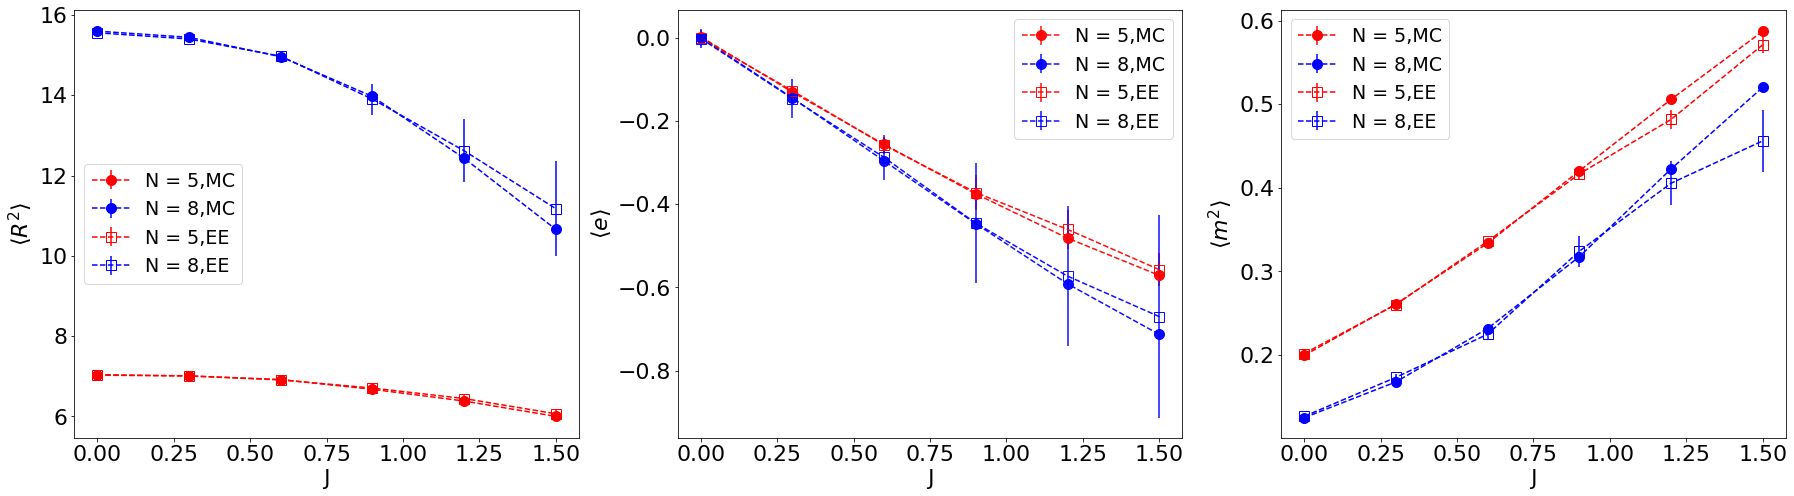
\includegraphics[scale=0.26]{Images/EE.png}
	\caption{$h=0$. Mean Radius \eqref{endtoend}, mean energy \eqref{hamiltonian} and   second moment of magnetization \eqref{secondmomentmagnetization}.   }
	\label{fig:ee}
\end{figure}


\subsection{Thermodynamics and structural properties, short chains}
To perform MC simulations for short chains from $N=100$ to $N=1000$, we run $4 \times 10^8$ MC steps for achieving equilibrium and at least $2.1 \times 10^9$ MC steps for measuring properties of the model.
 \begin{figure}[H]
	\centering
	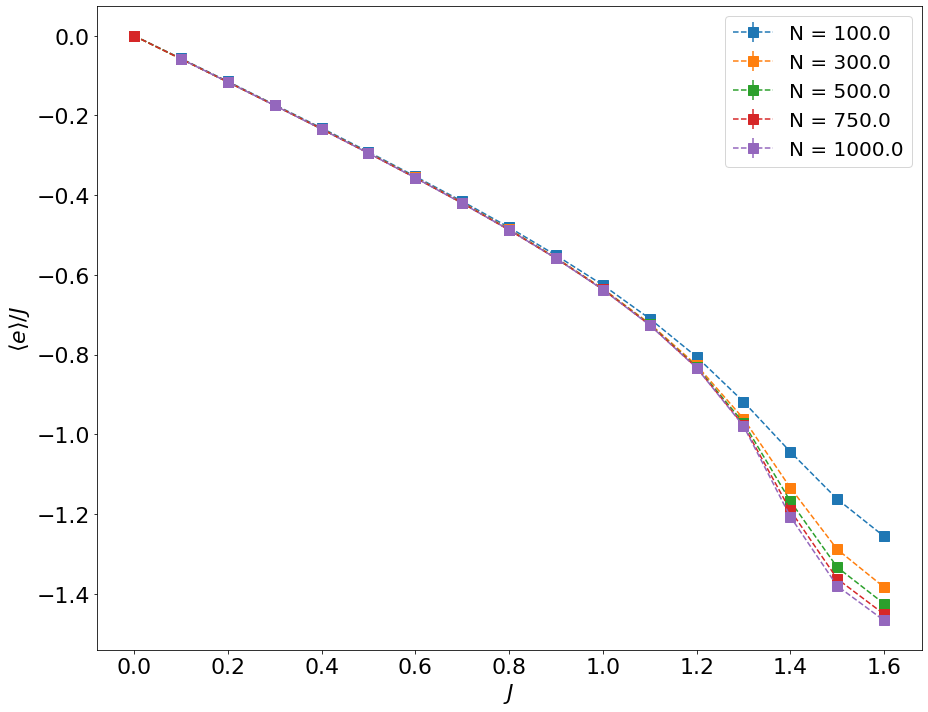
\includegraphics[scale=0.21]{Images/energy_shortchains.png}
	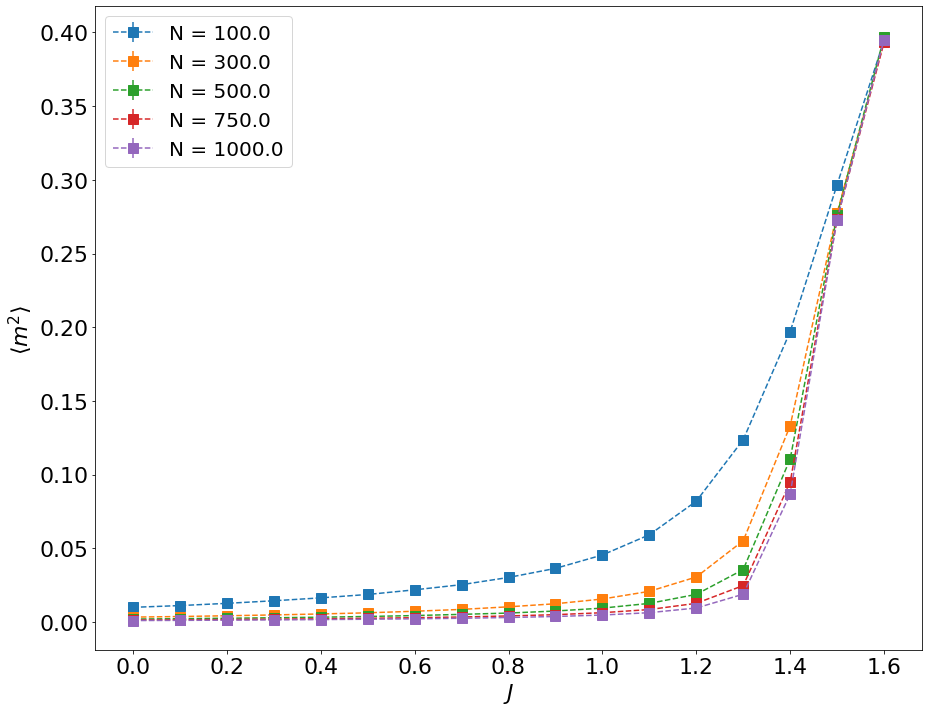
\includegraphics[scale=0.21]{Images/magnetization2_shortchains.png}
	\caption{$h=0$. Mean energy \eqref{hamiltonian} and   second moment of magnetization \eqref{secondmomentmagnetization} for short chains. $ > 4 \times 10^{9} $ MC steps in each simulations with two  types of updates: snake-like and reconnect.    }
	\label{fig:energymagshort}
\end{figure}

Figure \ref{fig:energymagshort} illustrates obtained results for Mean energy \eqref{hamiltonian} and   second moment of magnetization \eqref{secondmomentmagnetization} for short chains. The system tends to order as interaction energy $J$ gets larger. 

Next, we estimate critical exponent $\nu$. We use following ansatz  \cite{Berretti1985}:
\begin{equation}
\label{berettiscale}
\log (R_N^2+k_1 ) = 2 \nu \log (N+k_2) + b.
\end{equation}
Here $k_1=k_2=1$ are phenomenological parameters. 
 \begin{figure}[H]
	\centering
	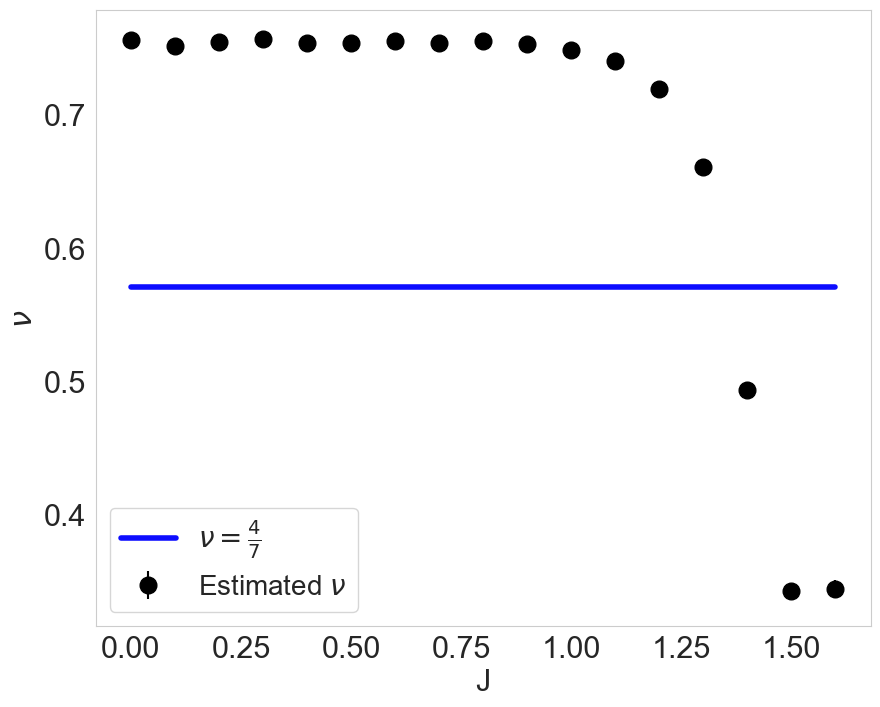
\includegraphics[scale=0.36]{Images/nu_shortchains.png}
	\caption{$h=0$. Estimations with errorbars of critical exponent $\nu$ .   }
	\label{fig:nushort}
\end{figure}
From figure \ref{fig:nushort}, we can assume that XY model on SAWs also has value $\nu = 4/7$ \eqref{nu_theta} at the point os structural phase transition. We use this value to obtain collapsing plots. 
 \begin{figure}[H]
 	\centering
 	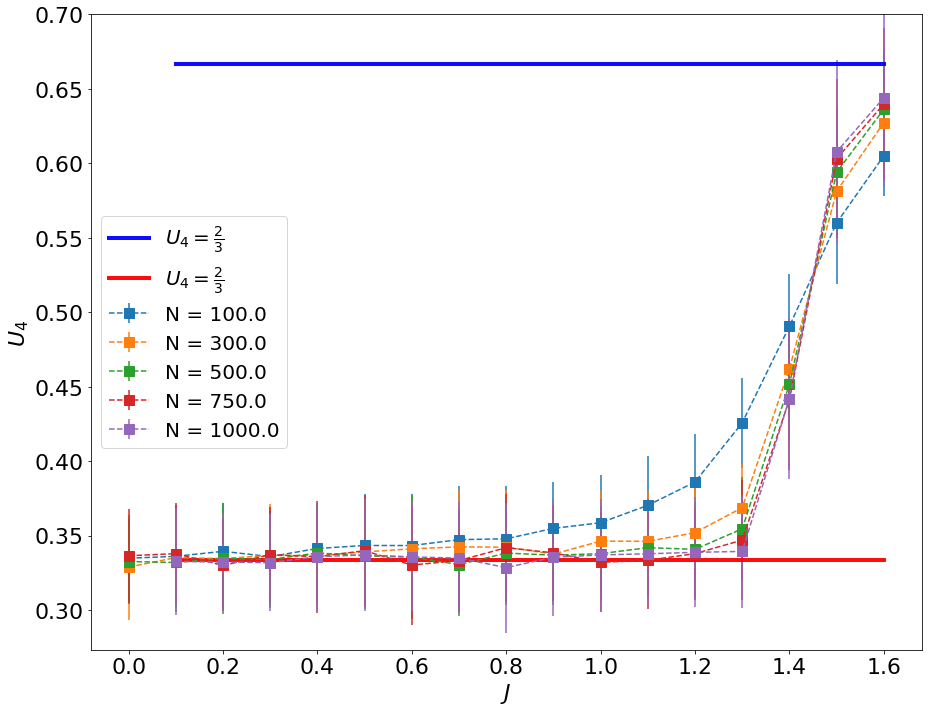
\includegraphics[scale=0.36]{Images/bindercumulants_shortchains.png} \\
 	 	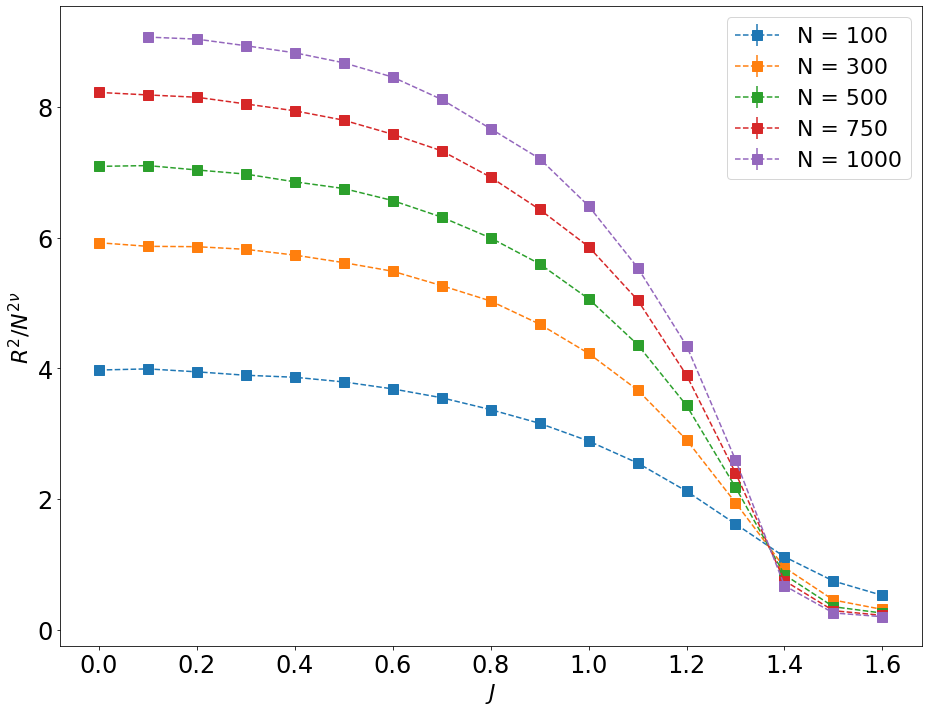
\includegraphics[scale=0.36]{Images/rscaling_shortchains.png}
 	\caption{$h=0$. Binder  cumulants \eqref{binderqum} and mean radius \eqref{endtoend} for short chains. $ > 4 \times 10^{9} $ MC steps in each simulations with two  types of updates: snake-like and reconnect.    }
 	\label{fig:bcshort}
 \end{figure}
 